\chapter{Proposta e Plano de Continuidade}
\label{ch:propos}

Neste capítulo é apresentada a proposta deste trabalho, com os requisitos, estórias de usuário, casos de uso e demais artefatos
que fazem parte do levantamento de requisitos e análise, oferecendo uma visão ampla da aplicação que será desenvolvida.
Além disso, também é apresentado o plano de continuidade com o cronograma para realização das etapas da segunda parte deste
trabalho.

\section{Descrição do Projeto}

Este projeto está sendo desenvolvido em parceria com a mestranda, Débora Almeida Silveira Sobral, do
Programa de Pós-graduação Profissional em Gestão e Inovação Tecnológica em Saúde (PPGITS), também orientanda da Profa.
Dra. Adicinéia Aparecida de Oliveira. E tem como objetivo
o desenvolvimento de uma aplicação móvel como ferramenta de auxilio à educação e ao autocuidado de pacientes diabéticos
com acuidade visual prejudica, acessível à PDV\@.

Para tanto, em \citeonline{Sobral2021} foi realizado um levantamento de referencial teórico e tecnológico sobre o DM,
aplicativos móveis e deficiência visual. Assim, reunindo as principais funcionalidades e soluções que o aplicativo a ser
desenvolvido deveria adotar como requisitos para que atendesse às necessidades desse público-alvo.

\section{Descrição do Plano de Continuidade}

Para o desenvolvimento completo desse projeto é previsto a realização de 4 etapas, ao longo dos meses referentes ao segundo
período letivo de 2021 da Universidade Federal de Sergipe (UFS), estas são listadas a seguir:
\begin{itemize}
    \item Desenvolvimento do aplicativo com a implementação dos requisitos mais essenciais e viáveis;
    \item Revisão e testes da acessibilidade da aplicação;
    \item Descrição do processo metodológico e análise dos resultados;
    \item Revisão, correção e entrega do trabalho.
\end{itemize}

\section{Busca de Anterioridade}

Em \citeonline{Sobral2021}, realizou-se uma busca de anterioridade, na base do Instituto Nacional de Propriedade Industrial (INPI)
e nas lojas de aplicativos Google Play (Android) e Apple Store (iOS), visando identificar os \emph{softwares} e funcionalidades
já existentes sobre DM e DV no mercado.
Assim, a \autoref{tab_cor_func} relaciona os \emph{apps} encontrados
nas lojas de aplicativos às principais funcionalidades propostas em seu trabalho para o DiaVision.

\begin{table}[htb]
    \caption{\label{tab_cor_func}Relação de funcionalidades dos \emph{apps} encontrados nas lojas de aplicativos.}
    \begin{center}
        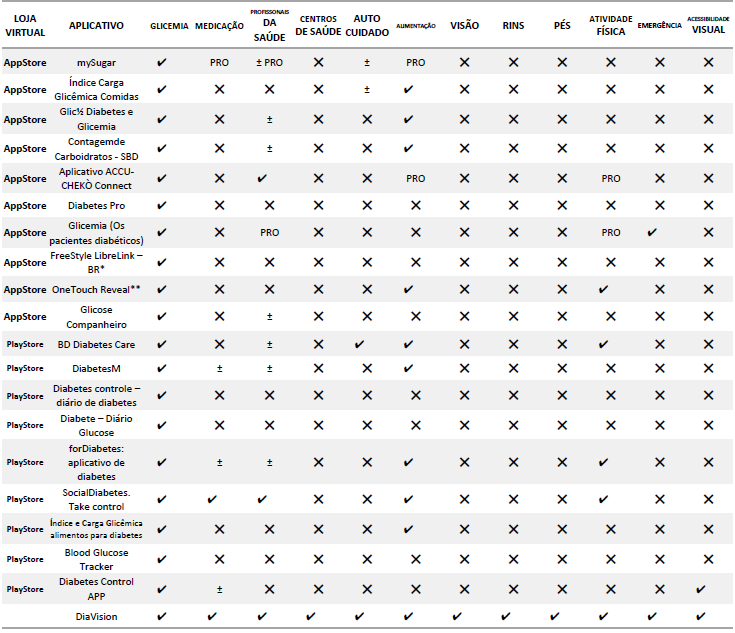
\includegraphics[scale=0.75]{Imagens/proposta/busca_anterioridade.png}
    \end{center}
    \legend{Fonte: \cite{Sobral2021}.}
\end{table}

\newpage

\section{Visão e Análise}

Nesta seção são descritas as necessidades e características esperadas do produto de \emph{software} a ser desenvolvido, identificadas a partir de
reuniões com a dona do produto (PO, do inglês \emph{product owner}), esta que identificou a problemática abordada neste trabalho e
realizou o levantamento de funcionalidades e problemas das soluções já existentes no mercado em \citeonline{Sobral2021}.

\subsection{Descrição do Problema}

A \autoref{tab-desc-pro} apresenta, de forma resumida, o problema, seus impactos e a proposta de solução com seu diferencial.

\begin{table}[htb]
    \caption{Descrição do problema.}
    \label{tab-desc-pro}
    \begin{center}
        \begin{tabular}{p{4.0cm}|p{10.0cm}}
            \textbf{Problema}    & Dificuldade de acesso à informações de autocuidado com relação ao DM por deficientes visuais.                                          \\
            \hline
            \textbf{Afeta}       & Independência e qualidade de vida de diabéticos com DV\@.                                                                              \\
            \hline
            \textbf{Impacta}     & No autocuidado e, consequentemente, no controle do DM\@.                                                                               \\
            \hline
            \textbf{Solução}     & Desenvolvimento de aplicação móvel com conteúdos e funcionalidades que auxiliem diabéticos no gerenciamento do autocuidado com o DM\@. \\
            \hline
            \textbf{Diferencial} & Acessibilidade ao deficiente visual.
        \end{tabular}
    \end{center}
    \legend{Fonte: Autores.}
\end{table}

\subsection{Riscos e Impedimentos}

Os seguintes riscos e possíveis impedimentos com relação ao produto foram identificados:

\begin{itemize}
    \item Não adesão por parte do público alvo;
    \item Dificuldades no manuseio do \emph{smartphone} pelo público alvo;
    \item Dificuldade de localizar os possíveis participantes da pesquisa;
    \item Utilização incorreta do aplicativo ou não assimilação das informações adquiridas;
    \item Afastamento do paciente da assistência continuada na rede primária;
    \item Constrangimento do usuário por falta de entendimento das funcionalidades.
\end{itemize}

\newpage

\section{Requisitos}

Antes de inciar o desenvolvimento de qualquer tarefa técnica de engenharia de \emph{software}, é interessante que seja criado
um conjunto de requisitos.
Isso porque as tarefas de levantamento de requisitos levam a um entendimento dos impactos da solução, necessidades do cliente e
como os usuários finais vão interagir com o \emph{software}, diminuindo as chances de erros por má interpretação das solicitações
dos clientes \cite{pressman2014software}.

Esses requisitos costumam ser classificados como funcionais, não-funcionais e inversos \cite{sommerville2007engenharia}.
E serão apresentados nesta seção, iniciando pelas estórias de usuários, parte inicial do processo de elicitação
dos requisitos e finalizando com os casos de uso.

\newpage

\subsection{Estórias de usuários}

Estórias de usuários são muito utilizadas em metodologias ágeis e descrevem um cenário geral no qual é possível visualizar
quais ações são possíveis, os atores envolvidos e quais os valores dessas ações, servindo como lembrete
de possíveis requisitos que precisam ser melhor detalhados com o cliente \cite{nawrocki2014agile}.

As estórias de usuários identificadas são listadas na \autoref{tab-est-usr}.

\begin{table}[htb]
    \begin{center}
        \ABNTEXfontereduzida
        \caption{Relação de estórias de usuários.}
        \label{tab-est-usr}
        \begin{tabular}{p{2.0cm}|p{5.0cm}|p{7.0cm}}
            %\hline
            \textbf{Eu, enquanto}                                          & \textbf{Quero} & \textbf{Para}                     \\
            \hline
            Paciente                                                       &
            Encontrar o \emph{app} nas lojas virtuais                      &
            Baixar o \emph{app} no meu celular.                                                                                 \\
            \hline
            Paciente                                                       &
            Realizar cadastro no aplicativo                                &
            Ter acesso às funcionalidades do \emph{app}.                                                                        \\
            \hline
            Paciente                                                       &
            Realizar login de forma prática                                &
            Para acessar as funcionalidades do \emph{app}.                                                                      \\
            \hline
            Paciente                                                       &
            Poder alterar minha senha                                      &
            Poder alterá\@-la e recuperar acesso ao \emph{app}.                                                                 \\
            \hline
            Paciente                                                       &
            Registrar informações das refeições                            &
            Acompanhar a quantidade de calorias consumidas por refeição.                                                        \\
            \hline
            Paciente                                                       &
            Ter acesso a aplicativos acessíveis para deficientes visuais   &
            Ajudar a realizar atividades do dia a dia.                                                                          \\
            \hline
            Paciente                                                       &
            Sugerir aplicativos acessíveis para deficientes visuais        &
            Compartilhar aplicativos que possam ajudar outros usuários com DV\@.                                                \\
            \hline
            Paciente                                                       &
            Registrar práticas de atividade física                         &
            Acompanhar a evolução da rotina de atividade física.                                                                \\
            \hline
            Paciente                                                       &
            Ter acesso à dicas de autocuidado                              &
            Melhorar a qualidade de vida e prevenir complicações do DM\@.                                                       \\
            \hline
            Paciente                                                       &
            Filtrar as dicas por categorias                                &
            Facilitar a busca das dicas sobre assuntos específicos.                                                             \\
            \hline
            Paciente                                                       &
            Consultar locais para acesso à serviços de saúde               &
            Facilitar o acesso e contato com as principais clínicas, hospitais e consultórios da cidade.                        \\
            \hline
            Paciente                                                       &
            Registrar glicemia                                             &
            Acompanhamento dos valores de glicemia e ser alertado quando estiver fora do limite.                                \\
            \hline
            Paciente                                                       &
            Registrar medicações que faço uso                              &
            Ter uma lista atualizada com todas as informações das medicações e ser alertado dos horários de uso das medicações. \\
            \hline
            Paciente                                                       &
            Realizar avaliação dos pés                                     &
            Acompanhar a evolução dos pés e detectar quando surgir alterações.                                                  \\
            \hline
            Paciente                                                       &
            Registrar diurese diária                                       &
            Acompanhar quando surgir alterações.                                                                                \\
            \hline
            Paciente                                                       &
            Ter acesso a relatórios dos dados registrados                  &
            Visualizar e compartilhar esses dados registrados.                                                                  \\
            \hline
            Paciente                                                       &
            Ter acesso aos dados pessoais                                  &
            Editar ou acrescentar dados pessoais durante o uso do aplicativo.                                                   \\
            \hline
            Paciente                                                       &
            Configurar notificações                                        &
            Definir horários e quais ativar ou desativar.                                                                       \\
            \hline
            Paciente                                                       &
            Configurar preferências                                        &
            Personalizar os limites da glicemia.                                                                                \\
            \hline
            Paciente                                                       &
            Realizar \emph{logout}                                         &
            Para desvincular minha conta do \emph{app}.                                                                         \\
            \hline
            Administrador do sistema                                       &
            Adicionar dicas de autocuidado para os pacientes               &
            Fornecer informações acerca de cuidados com a saúde.                                                                \\
            \hline
            Administrador do sistema                                       &
            Cadastrar centros de saúde no sistema                          &
            Que o paciente possa conhecer os centros de saúde que atendem suas demandas.                                        \\
            \hline
            Administrador do sistema                                       &
            Cadastrar sugestões de aplicativos acessíveis no sistema       &
            Que o paciente possa conhecer outros \emph{apps} acessíveis que possam ajudá\@-lo no cotiano.                       \\
            \hline
            Administrador do sistema                                       &
            Aprovar/recusar as sugestões de centros de saúde e aplicativos &
            Assegurar credibilidade ao aplicativo.                                                                              \\
            % \hline
        \end{tabular}
        \legend{Fonte: Autores.}
    \end{center}
\end{table}

\newpage

\subsection{Requisitos Funcionais}

A \autoref{tab-req-fun} mostra os requisitos funcionais da aplicação, estes que se referem, principalmente, às funções e 
comportamentos do sistema.

\begin{table}[htb]
    \begin{center}
        \ABNTEXfontereduzida
        \caption{Requisitos Funcionais da aplicação.}
        \label{tab-req-fun}
        \begin{tabular}{p{1.1cm}|p{1.3cm}|p{3.0cm}|p{1.5cm}|p{6.7cm}}
            %\hline
            \textbf{Código} & \textbf{Atores} & \textbf{Requisito}              & \textbf{Prioridade} & \textbf{Descrição} \\
            \hline
            RF01            & Paciente        & Manter paciente                 & Essencial           &
            O paciente poderá gerenciar seus dados na aplicação.                                                           \\
            \hline
            RF02            & Paciente        & Resetar senha                   & Essencial           &
            O paciente poderá solicitar a alteração de senha para recuperar acesso.                                        \\
            \hline
            RF03            & Paciente        & Autenticação                    & Essencial           &
            Será necessária autenticação com e-mail e senha para ter acesso às funcionalidades do \emph{app}.              \\
            \hline
            RF04            & Adminis-trador  & Manter Dicas de Autocuidado     & Essencial           &
            O administrador do sistema poderá gerenciar as dicas de autocuidado no sistema.                                \\
            \hline
            RF05            & Adminis-trador  & Manter Centros de Saúde         & Desejável           &
            O administrador do sistema poderá gerenciar os centros de saúde no sistema.                                    \\
            \hline
            RF06            & Adminis-trador  & Manter \emph{Apps} de Visão     & Importante          &
            O administrador do sistema poderá gerenciar sugestões de aplicativos acessíveis à PDV\@.                       \\
            \hline
            RF07            & Paciente        & Manter Registros de Diurese     & Importante          &
            O paciente poderá registrar diurese e gerenciar esses registros.                                               \\
            \hline
            RF08            & Paciente        & Manter Registros de Glicemia    & Essencial           &
            O paciente poderá registrar níveis de glicemia e gerenciar esses registros.                                    \\
            \hline
            RF09            & Paciente        & Manter Registros de Medicação   & Essencial           &
            O paciente poderá registrar suas medicações e gerenciar esses registros.                                       \\
            \hline
            RF10            & Paciente        & Manter Registros de Exercícios  & Importante          &
            O paciente poderá registrar atividades físicas realizadas e gerenciar esses registros.                         \\
            \hline
            RF11            & Paciente        & Manter Avaliações dos Pés       & Essencial           &
            O paciente poderá registrar avaliações do estado dos pés e gerenciar esses registros.                          \\
            \hline
            RF12            & Paciente        & Sugerir \emph{Apps} de Visão    & Importante          &
            O paciente poderá sugerir de aplicativos acessíveis à PDV para avaliação do administrador.                     \\
            \hline
            RF13            & Paciente        & Manter Registros de Alimentação & Essencial           &
            O paciente poderá registrar os alimentos que consumiu por refeição e gerenciar esses registros.                \\
            \hline
            RF14            & Paciente        & Consultar Dicas de Autocuidado  & Essencial           &
            O paciente poderá consultar as dicas de autocuidado disponíveis no sistema.                                    \\
            \hline
            RF15            & Paciente        & Consultar Centros de Saúde      & Desejável           &
            O paciente poderá consultar os centros de saúde disponíveis no sistema.                                        \\
            \hline
            RF16            & Paciente        & Consultar \emph{Apps} de Visão  & Importante          &
            O paciente poderá consultar sugestões de aplicativos acessíveis à PDV\@ disponíveis no sistema.                \\
            \hline
            RF17            & Paciente        & Sugerir Centros de Saúde        & Desejável           &
            O paciente poderá sugerir centros de saúde para avaliação do administrador.                                    \\
            \hline
            RF18            & Paciente        & Configurar Notificações         & Essencial           &
            O paciente poderá configurar quais notificações deseja receber e os horários.                                  \\
            \hline
            RF19            & Paciente        & Envio de Notificações           & Essencial           &
            Notificações deverão ser enviadas de acordo com as configurações definidas pelo paciente.                      \\
            % \hline
        \end{tabular}
        \legend{Fonte: Autores.}
    \end{center}
\end{table}

\newpage

\subsection{Requisitos Não-Funcionais}

Requisitos não-funcionais em sistemas podem ser descritos como atributos de qualidade, desempenho, segurança ou gerais, estes que podem
ser identificados a partir das necessidades do cliente mesmo que não tenham sido falados explicitamente \cite{pressman2014software}.

Assim, na \autoref{tab-req-nf}, são listados esses requisitos identificados juntamente com o tipo e a prioridade
de cada um deles para este projeto.

\begin{table}[htb]
    \begin{center}
        \ABNTEXfontereduzida
        \caption{Requisitos Não-Funcionais da aplicação.}
        \label{tab-req-nf}
        \begin{tabular}{p{1.1cm}|p{1.6cm}|p{3.0cm}|p{1.5cm}|p{6.7cm}}
            %\hline
            \textbf{Código} & \textbf{Tipo} & \textbf{Requisito}              & \textbf{Prioridade} & \textbf{Descrição} \\
            \hline
            RNF01           & Usabilidade   & Acessibilidade                  & Essencial           &
            Implementar as técnicas de acessibilidade para solucionar os principais problemas relacionados.              \\
            \hline
            RNF02           & Usabilidade   & Simplicidade                    & Essencial           &
            \emph{Interface} simples e intuitiva, mantendo apenas as informações necessárias na tela.                    \\
            \hline
            RNF03           & Usabilidade   & Buscas Ágeis                    & Desejável           &
            Facilitar buscas por meio de \emph{auto complete}.                                                           \\
            \hline
            RNF04           & Segurança     & Compartilhamento de Informações & Essencial           &
            Somente o próprio usuário terá acesso e poderá compartilhar suas informações.                                \\
            \hline
            RNF05           & Tecnologia    & Aplicação multiplataforma       & Desejável           &
            Deve-se utilizar de ferramentas que possibilitem a construção da aplicação para Android e iOS\@.             \\
            % \hline
        \end{tabular}
        \legend{Fonte: Autores.}
    \end{center}
\end{table}

\subsection{Requisitos Inversos}

Os requisitos listados na \autoref{tab-req-inv}, chamados inversos, se referem às restrições, condições que não devem ocorrer no sistema.

\begin{table}[htb]
    \begin{center}
        \ABNTEXfontereduzida
        \caption{Requisitos Inversos da aplicação.}
        \label{tab-req-inv}
        \begin{tabular}{p{1.1cm}|p{1.5cm}|p{10.5cm}}
            %\hline
            \textbf{Código} & \textbf{Prioridade} & \textbf{Descrição}         \\
            \hline
            RI01            & Essencial           &
            Um usuário não deve poder acessar recursos de outros.              \\
            \hline
            RI02            & Essencial           &
            Os usuários não devem ser notificados se não estiverem deslogados. \\
            \hline
            RI03            & Essencial           &
            O administrador do sistema não deve ter acesso aos dados dos usuários.
            % \hline
        \end{tabular}
        \legend{Fonte: Autores.}
    \end{center}
\end{table}

\newpage

\subsection{Casos de Uso}

De acordo com \citeonline{pressman2014software}, um caso de uso é caracterizado como um ``contrato de comportamento'' que define como
um ator utiliza um sistema para alcançar algum objetivo e descreve um cenário de uso de forma simples do ponto de vista desse ator.

A partir dos requisitos e estórias de usuários identificados, o diagrama de casos de usos da \autoref{fig_use_cas} foi elaborado.

\begin{figure}[htb]
    \caption{\label{fig_use_cas}Diagrama de casos de uso.}
    \begin{center}
        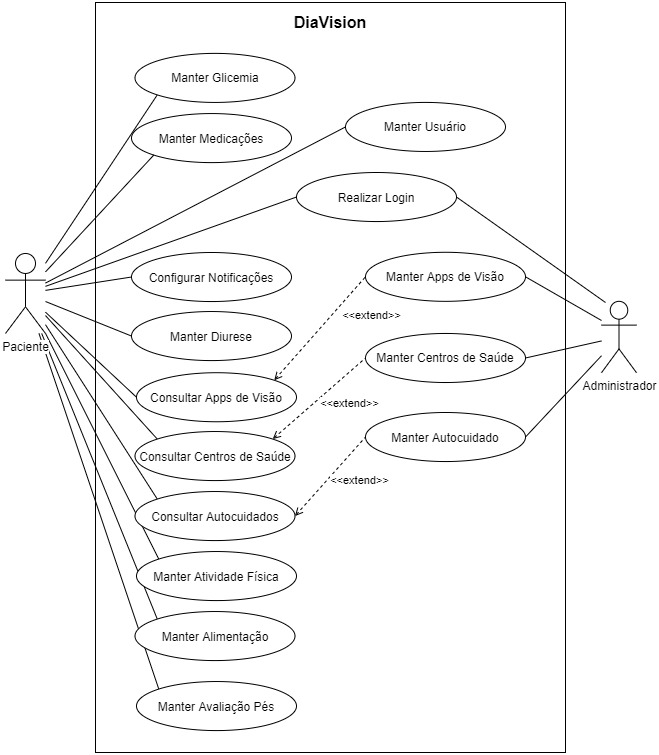
\includegraphics[scale=0.65]{Imagens/proposta/use_case.jpg}
    \end{center}
    \legend{Fonte: Autor.}
\end{figure}

\newpage

\section{Protótipo de Telas}

Nesta seção são apresentadas imagens do protótipo de telas elaborado no estudo \citeonline{Sobral2021}, com o objetivo de melhorar o entendimento dos
requisitos e funcionalidades do aplicativo que será desenvolvido.
Assim, nas \autoref{fig_tel_ini_prot} e \autoref{fig_tel_pos_prot} são mostradas as telas iniciais e demais telas do protótipo.

\begin{figure}[htb]
    \caption{\label{fig_tel_ini_prot}Telas iniciais do protótipo.}
    \begin{center}
        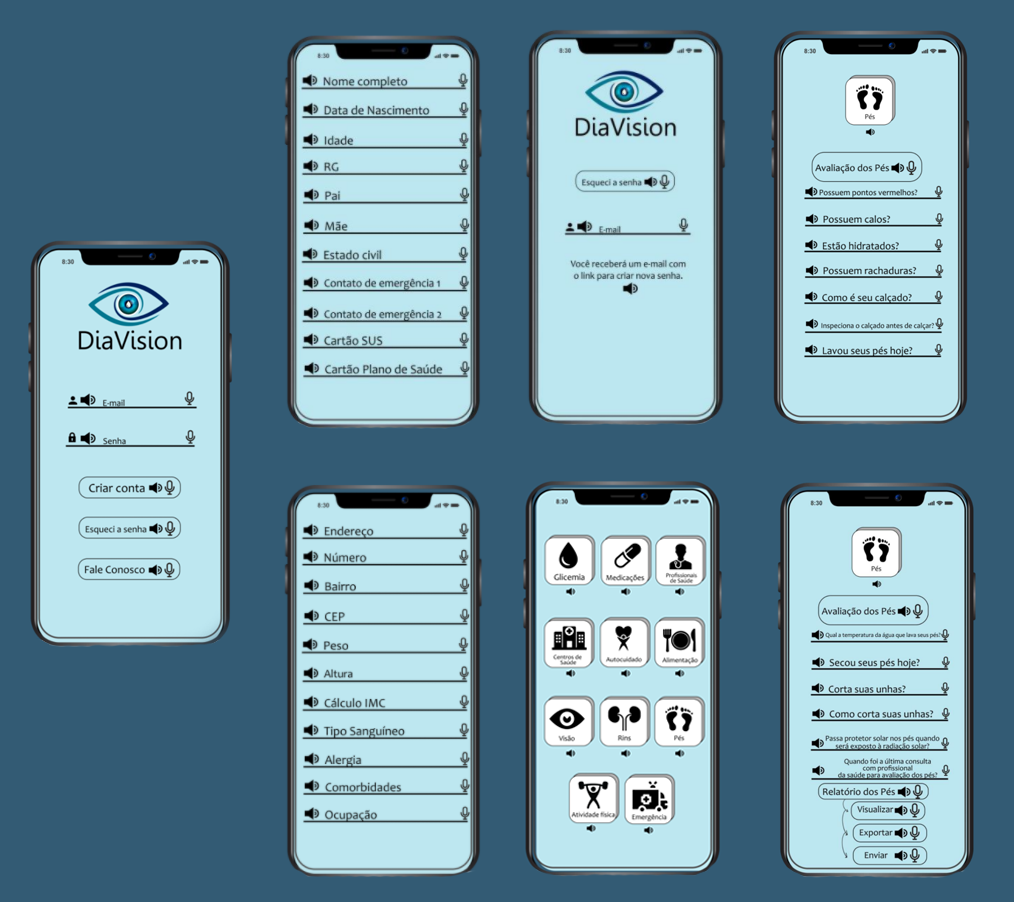
\includegraphics[scale=0.57]{Imagens/proposta/telas_iniciais_prot.png}
    \end{center}
    \legend{Fonte: \cite{Sobral2021}.}
\end{figure}

\begin{figure}[htb]
    \caption{\label{fig_tel_pos_prot}Demais telas do protótipo.}
    \begin{center}
        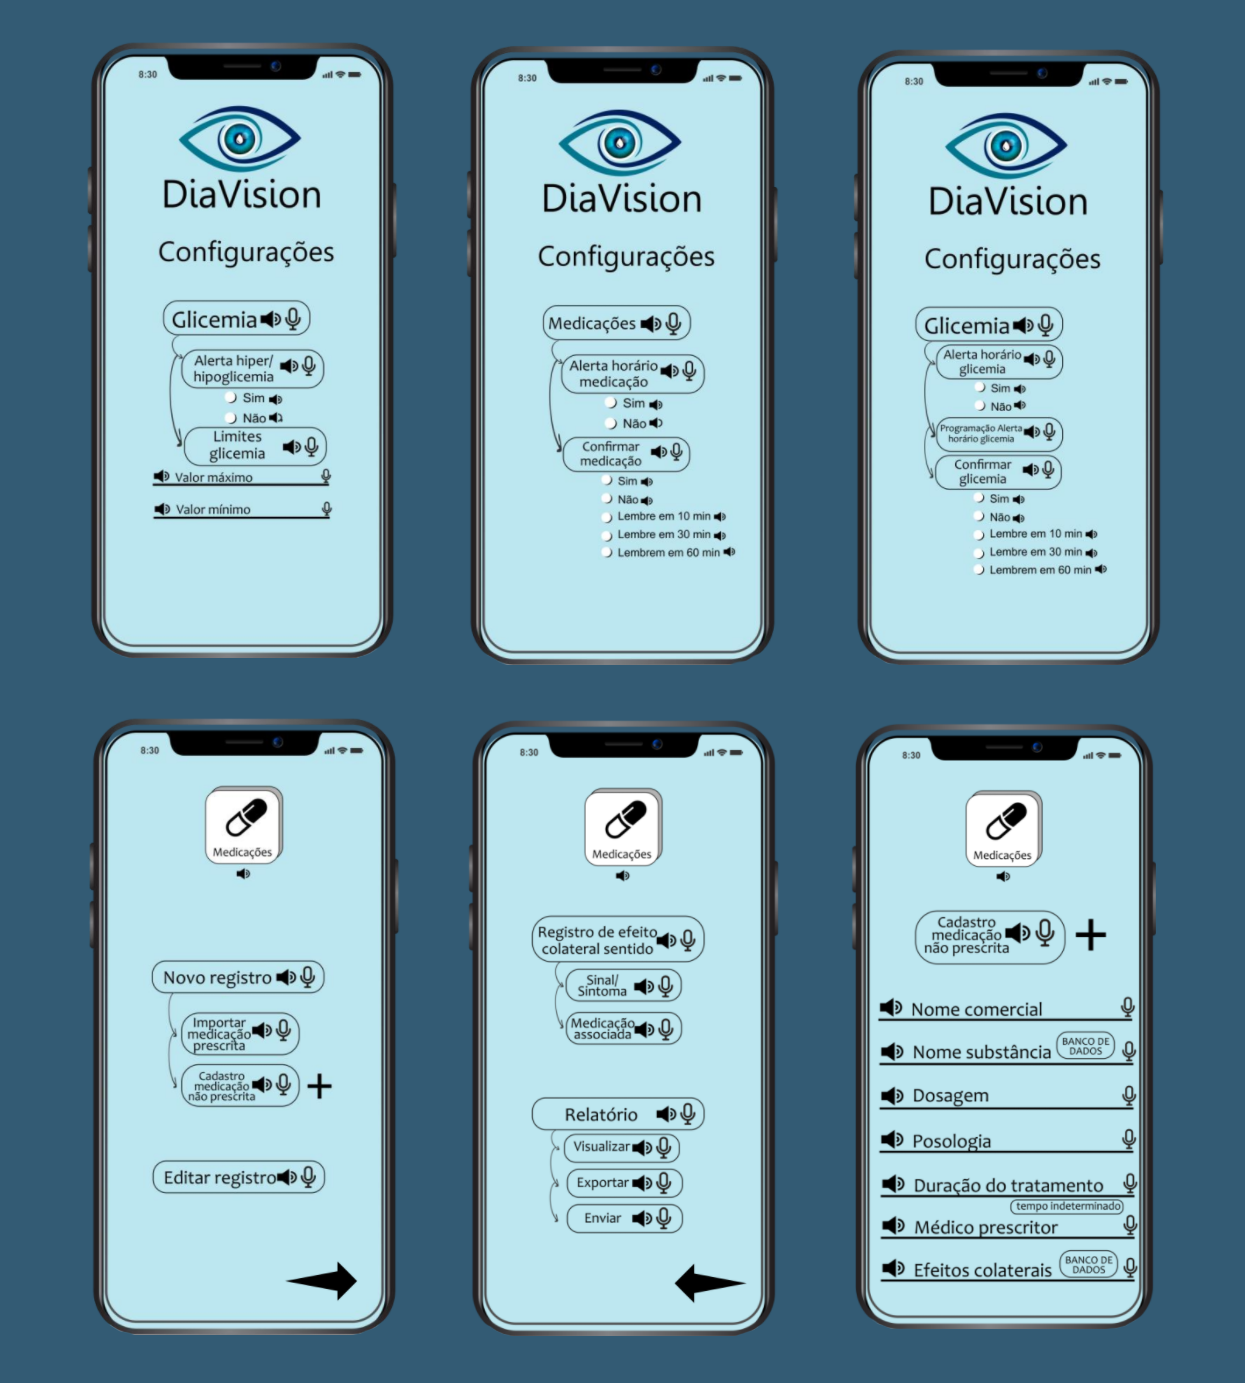
\includegraphics[scale=0.45]{Imagens/proposta/telas_post_prot.png}
    \end{center}
    \legend{Fonte: \cite{Sobral2021}.}
\end{figure}

\newpage

\section{Cronograma}

Por fim, o cronograma na \autoref{fig_cro_con} foi definido visando a organização e planejamento das atividades que serão realizadas
na segunda parte desse trabalho.

\begin{figure}[htb]
    \caption{\label{fig_cro_con}Cronograma de continuidade do Projeto.}
    \begin{center}
        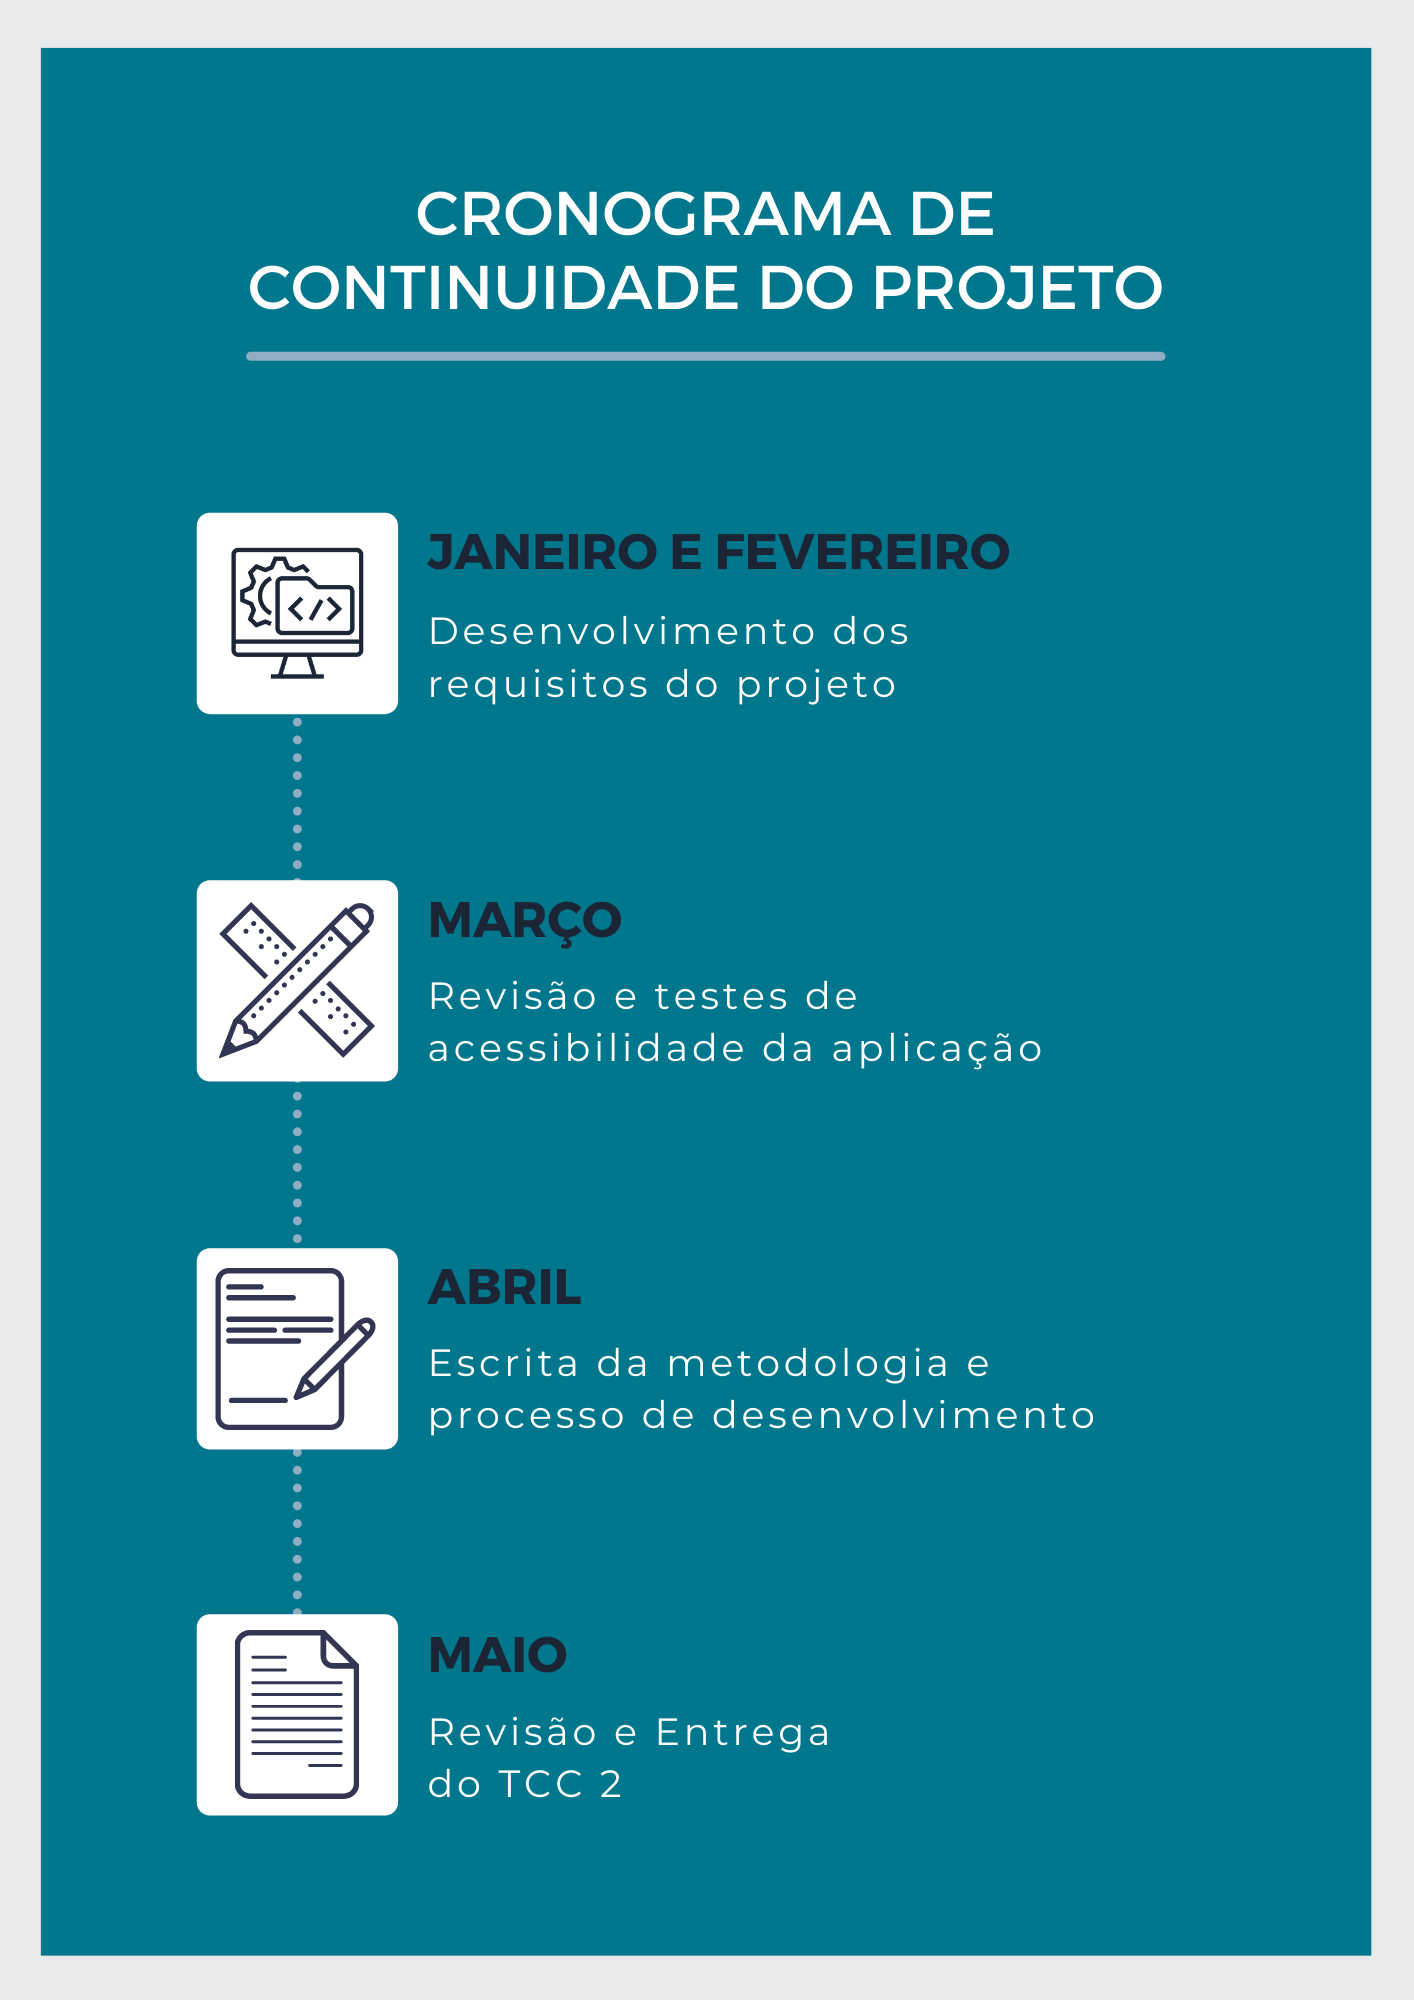
\includegraphics[scale=0.65]{Imagens/proposta/cronograma_continuidade.png}
    \end{center}
    \legend{Fonte: Autor.}
\end{figure}